\section{Hardware Implementation\label{sec:Hardware-Implementation}}


\subsection{Methodology}

Commonality between modules, same life-support system.


\subsection{CAD Design}

Schematic capture and PCB layout using EagleCAD.


\subsection{Commonalities}

All 4 modules are implemented on custom printed circuit boards (PCBs) with an \emph{AT90CAN128} micro-controller from Atmel. Programming and debugging software on the microcontroller was done through a standard IEEE 1149.1 JTAG interface. The module is linked to the other system modules with a CAN bus. All inter-module communication is done over the CAN bus.

\subsubsection{Microcontroller}


\subsubsection{CAN Transceiver}


\subsubsection{Linear Regulator}


\subsubsection{Supervisor}


\subsubsection{Wiring Harness}


\subsection{Engine and Transmission Module}

\begin{figure}[h]
\centering
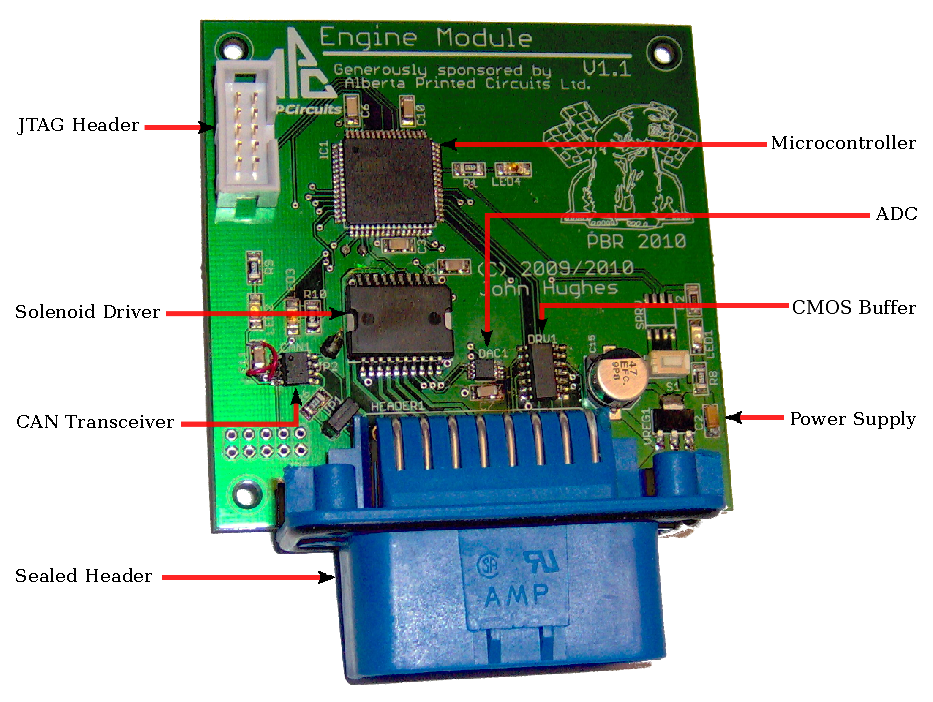
\includegraphics[scale=1]{implementation/figures/engine_transmission_pcb}
\caption{Populated Engine and Transmission module PCB.}
\label{fig:engine_transmission_pcb}
\end{figure}

In addition to the common life-support hardware for the micro-controller (such as the voltage regulator and decoupling capacitors), the engine module includes an SPI capable octal \emph{low-side solenoid driver}. This driver chip switches the low side of the solenoid valves, as well as the starter solenoid. It includes flyback protection circuitry to squash voltage spikes from the inductive load of the solenoid, and can also detect electrical shorts. 

\begin{table}
  \caption{Engine and Transmission module components.\label{table:engine_transmission_module_components}}
  \centering
  \begin{tabular}{|c|c|c|}
    \hline 
    Part & Manufacturer & Part Number\tabularnewline 
    \hline \hline
    Solenoid Driver & ST Microelectronics & L9822E \tabularnewline
    \hline
    Digital to Analogue Converter & Texas Instruments & TLV5623C \tabularnewline
    \hline
    Hex CMOS Buffer & Texas Instruments & 74LVC07A \tabularnewline
    \hline
  \end{tabular}
\end{table}


\subsubsection{High Current Solenoid Driver}

In order to meet the requirement of being able to energize the multiple solenoids specified in the design, an 8-way solenoid driver component from ST Microelectronics was chosen. The LT9822E provides a simple SPI interface for the microcontroller to talk to, and also takes care of possible flyback from the solenoids with built-in clamping diodes.

Using this single component strongly reduces the complexity of the output stage of the circuit, since multiple discrete high-current transistors were not needed.

\subsubsection{Input Buffers}


\subsubsection{Traction Control Analogue Output}

In order to generate a 0-5V analogue signal for the ECU's traction slip ratio input, as was described in Sec. \ref{sec:background_ecu_data_interfaces}, a simple SPI interfaced digital to analogue converter (DAC) from Texas Instruments was introduced. The TLV5623 outputs 0-5V analogue signal that varies with the digital input.

The output voltage from the DAC can be determined by the following equation:

\begin{equation}
V_{out}=2\cdot{V_{ref}}\,\frac{Code}{2^{n}}\,[V]
\end{equation}

where $V_{ref}$ is the reference voltage input to the chip, $n=8\,(bits)$, and $Code$ is the digital input value ranging from $0$ to $2^{n-1}$. Since we want to output $5\,[V]$ at fullscale input, \begin{equation} 2\cdot{V_{ref}}\,\frac{2^{7}}{2^{8}}=V_{ref}=5\,[V]\end{equation}.

The DC input resistance $R_{in}$ on the traction cut input pin on the ECU was measured using a series resistor with the input terminal to be $R_{in}\approx155k\Omega$. The output current of the DAC therefore will be at most $I_{out}=\frac{5v}{155k}\approx32.26\mu A$.

\subsection{Braking Module}

<Picture of board>


\subsubsection{Stepper Motor Driver}


\subsubsection{Analogue-to-Digital Converter}


\subsubsection{End-of-Travel Microswitches}

\subsection{Telemetry Module}


\subsubsection{Wireless Modem}

To meet the range and data throughput requirements for the telemetry system, an XBee Pro wireles modem was used. The XBee requires \unit{3.3}{\volt} I/O levels and power supply, and so a second linear voltage regulator was used in the design, the LT1521 from Linear Technology. Since the AT90CAN129 has only 2 built-in UARTS that were used for the RS232 interfaces to the ECU and DAQ, an third external UART was added to the design. The MAX3100 is a SPI-interfaced UART with an 8 word deep FIFO buffer. It is interfaced to the AT90CAN128's SPI pins and has an active-low IRQ line connected to external interrupt line EXT7 on the microcontroller. 

The wireless transmitter is an XBee Pro Modem from Digi International. The modem is in a package designed for mounting on a printed circuit board, and is attached to the telemetry module directly. This modems requires a 3.3V power supply. and consumes at most 215mA of current during transmit. Since the common module hardware only provides power for 5V devices, the telemetry module has a second LDO regulator providing 3.3V. A separate antenna port is connected to the modem and mounted in the side of the module enclosure.



\subsubsection{External SPI USART}


\subsubsection{Two-Channel ECU and DAC USART}

\input{implementation/implementation_hardware_driver_interface.tex}